\documentclass[a4paper]{article}

\title{PH2255 Course:\\
Introduction to Statistical Methods\\
Interference Patterns of Coherent Light\\in the Fraunhofer and Fresnel Regimes}
\author{Thomas Bass}
\date{25 Feb 2021}

% LaTeX preambule: loading relevant packages, configuring Python listings
\usepackage{graphicx}
\usepackage{amsmath}
\usepackage{color}
\usepackage{listings}
\usepackage{hyperref}
\usepackage{bm}
\usepackage{subcaption}
\usepackage[a4paper, total={6in, 8in}]{geometry}

\definecolor{dkgreen}{rgb}{0,0.6,0}
\definecolor{gray}{rgb}{0.5,0.5,0.5}
\definecolor{mauve}{rgb}{0.58,0,0.82}

% Settings for colour-coding and formatting Python code:
\lstset{
  language=Python,                % the language of the code
  basicstyle=\footnotesize,           % the size of the fonts that are used for the code
  numbers=left,                   % where to put the line-numbers
  numberstyle=\tiny\color{gray},  % the style that is used for the line-numbers
  stepnumber=5,                   % the step between two line-numbers. If it's 1, each line
                                  % will be numbered
  numbersep=5pt,                  % how far the line-numbers are from the code
  backgroundcolor=\color{white},      % choose the background color. You must add \usepackage{color}
  showspaces=false,               % show spaces adding particular underscores
  showstringspaces=false,         % underline spaces within strings
  showtabs=false,                 % show tabs within strings adding particular underscores
  frame=single,                   % adds a frame around the code
  rulecolor=\color{black},        % if not set, the frame-color may be changed on line-breaks within not-black text (e.g. commens (green here))
  tabsize=2,                      % sets default tabsize to 2 spaces
  captionpos=b,                   % sets the caption-position to bottom
  breaklines=true,                % sets automatic line breaking
  breakatwhitespace=false,        % sets if automatic breaks should only happen at whitespace
  title=\lstname,                   % show the filename of files included with \lstinputlisting;
                                  % also try caption instead of title
  keywordstyle=\color{blue},          % keyword style
  commentstyle=\color{dkgreen},       % comment style
  stringstyle=\color{mauve},         % string literal style
  escapeinside={\%*}{*)},            % if you want to add LaTeX within your code
  morekeywords={*,...}               % if you want to add more keywords to the set
}

\begin{document}
\maketitle

\begin{abstract}
It was long thought, and is common assumption, that light travels in straight lines. While this is largely true, when passing through small apertures - such that wavelength of light is actually significant compared to the dimensions of the aperture - one can observe interactions between light rays and the geometry of double and single slits, diffraction gratings, and pinhole apertures. To observe these interactions, we use a coherent light source - a laser - to shine beams of photons through varying aperture shapes, and observe the pattern of light behind them. To analyse these quantitatively, we employ techniques developed by Fraunhofer and Fresnel. These techniques describe two regimes of diffraction, the main difference being that the Fresnel regime requires the observation plane to be significantly closer to the source than Fraunhofer, or that the wavefronts of light have considerable curvature.
\end{abstract}
\section{Equipment}

Despite the experimental results being provided for this lab, it is important to understand how they were obtained. The apparatus consists of a Helium-Neon ($HeNe$) laser, of wavelength $623.8\ nm$, a Gambrell viewing screen, and an aperture and lens between them. The Gambrell viewing screen provides us with a white ruler, with millimetre markers, to easily and accurately measure the geometries of the diffraction pattern. The lens is a beam expansion lens, which expands the beams before hitting the Grambrell screen. This allows us to switch between the Fraunhofer and Fresnel diffraction regimes by including or removing the lens, changing the focal point of the system, instead of having to move the Gambrell screen backwards and forwards. 

\begin{figure}[h!]
\centerline{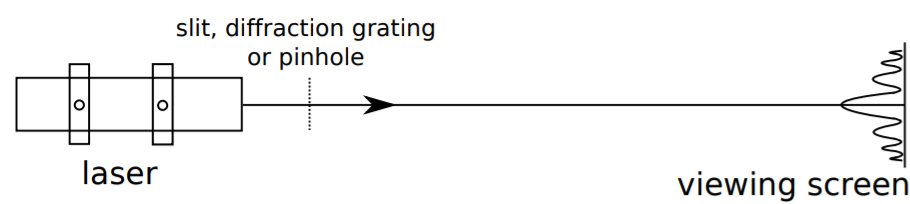
\includegraphics[scale=0.3]{setup.png}}%
\caption{Diagram showing the equipment setup.}
\label{fig:setup}
\end{figure}

\section{Single slit}
\subsection{Method}

In the Fraunhofer regime, we use phasor analysis to to sum the contributions of each infinitesimal element of the wavefront. Considering a single slit, the aperture function depends only on $x$, so we observe the intensity of light $I$ observed at angle $\theta$ as:

\begin{equation}
\frac{I(\theta)}{I_0}=\frac{sin^2\alpha}{\alpha^2}
\end{equation}

Where $\alpha=(\pi/\lambda)\cdot \alpha\sin\theta$. This follows the form of a $\text{sinc}^2 x$ plot, shown below for aperture gaps at 50, 100, and 200 $\mu m$:

\begin{figure}[h!]
\centerline{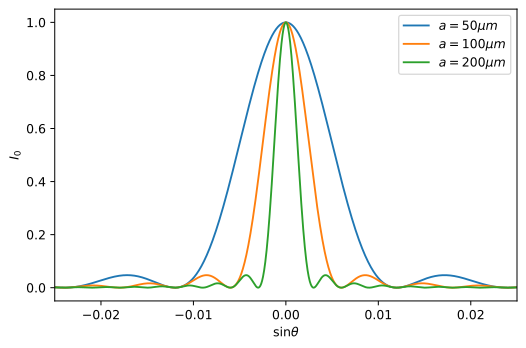
\includegraphics[scale=0.6]{demo.png}}%
\caption{Diagram showing the single-slit Fraunhofer diffraction patterns for 50, 100, and 200 $\mu m$. The plots follow a $\text{sinc}^2 x$ graph.}
\label{fig:demo}
\end{figure}

By identifying dark spots (interference minima) on an observed diffraction pattern, we can relate the horizontal offset $X$ of a minima to the angular difference from forwards, accounting for a small offset of $\Delta\theta$:

\begin{equation}
\frac XL=\tan(\theta+\Delta\theta)
\end{equation}
where $L$ is the distance between the slit and the screen. Knowing that we find these minima where $a\sin\theta=n\lambda$, and using the small angle approximations $\sin\theta\approx\tan\theta\approx\theta$, we obtain and equation describing the locations of the minima:

\begin{equation}
\frac XL=\frac\lambda an+\Delta\theta
\end{equation}
\newpage
\subsection{Data and Analysis}

By analysing the data provided, using \lstinline$Q2_slitA3.jpg$, we can identify the locations of minima between $N=-4$ and $N=4$, as well as identifying the offset $\Delta\theta$. Analysis of the photograph is found below.

\begin{figure}[h!]
\centerline{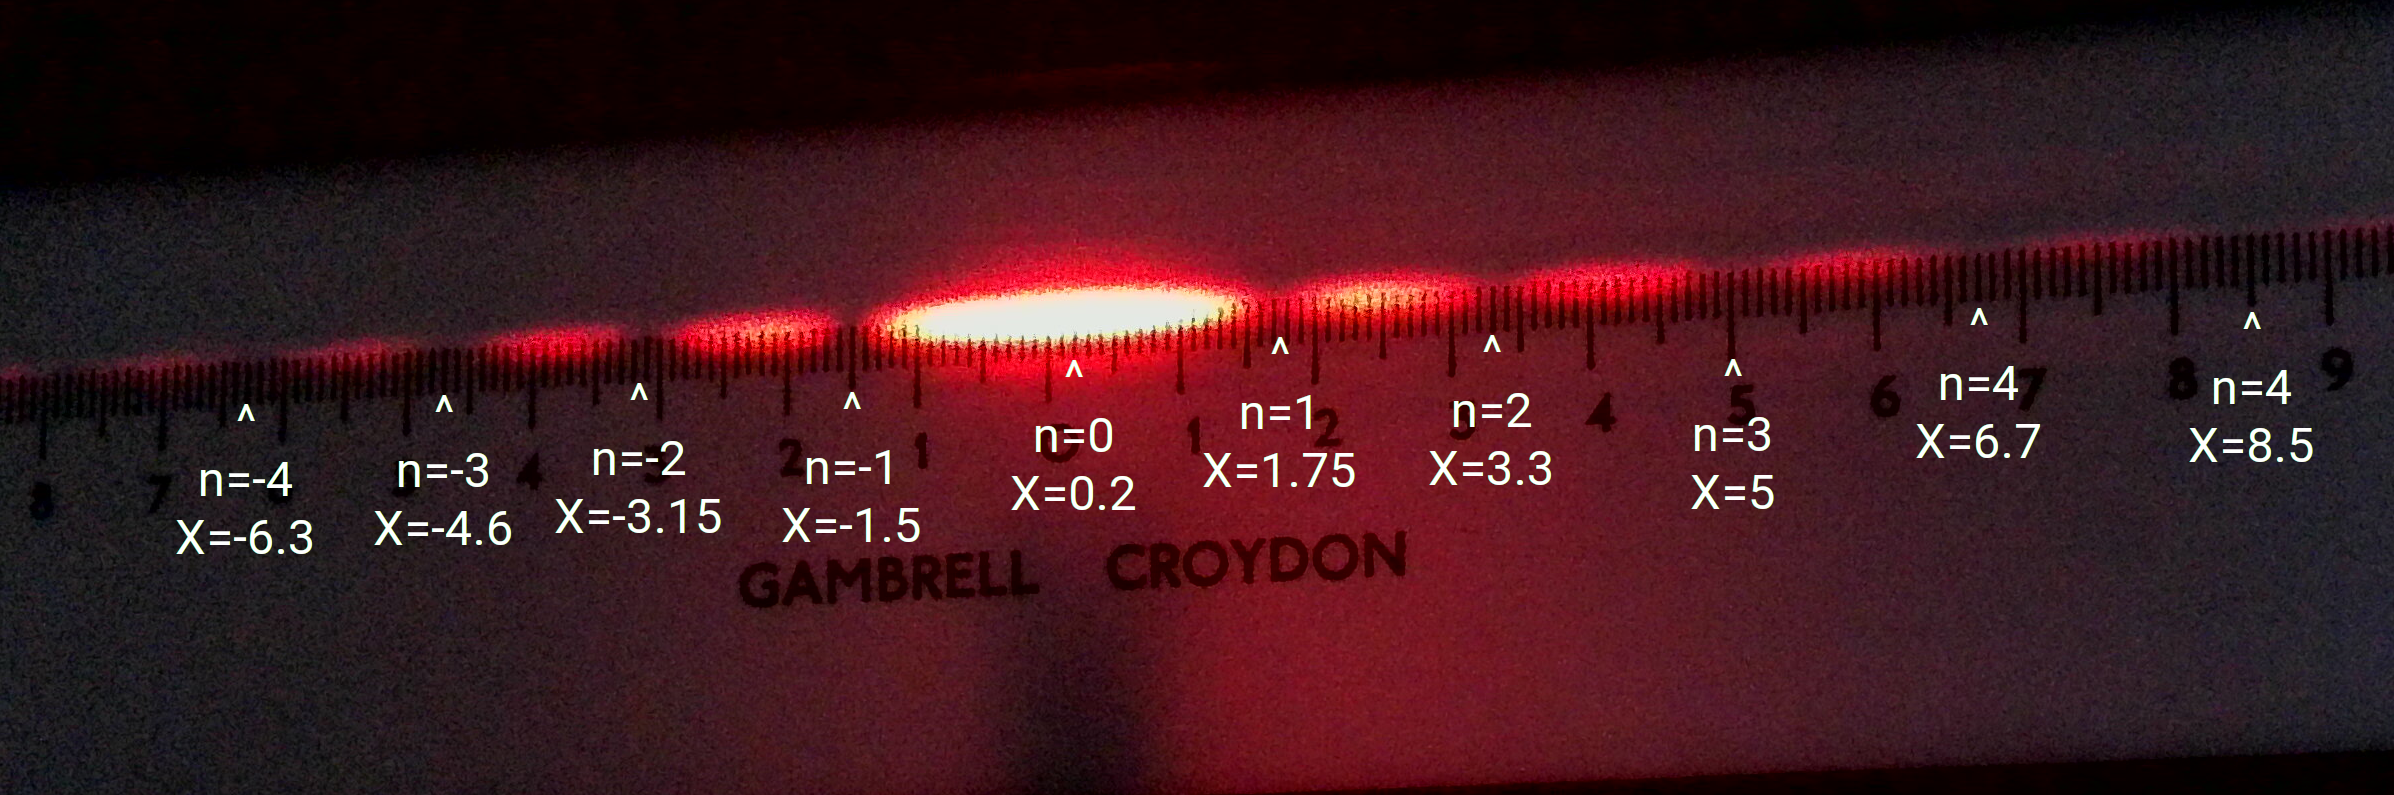
\includegraphics[scale=0.5]{L166pm1.png}}
\caption{Analysis of the data from image {\lstinline$Q2\_slitA3.jpg$}, identifying interference minima between $N=-4$ and $N=4$, as well as $N=0$ for the $\Delta\theta$ offset}
\label{fig:l116pm1}
\end{figure}

For this dataset, we are told that $L=166\pm1 \text{cm}$. From the analysis, we obtain the following data:

\begin{table}[h!]
\centering
\begin{tabular}{ccc}
\hline
N (order) & Minima position X (cm) & Uncertainty (cm)\\ \hline
-4 & -6.3 & 0.1 \\
-3 & -4.6 & 0.1 \\
-2 & -3.15 & 0.05 \\
-1 & -1.5 & 0.05 \\
0 & 0.2 & 0.1 \\
1 & 1.75 & 0.05 \\
2 & 3.3 & 0.05 \\
3 & 5.0 & 0.1 \\
4 & 6.7 & 0.1 \\
\end{tabular}
\caption{\label{tab:l116_table}Results from analysis of Figure \emph{3}}
\end{table}

We repeat this analysis for a second image in the data set, \lstinline$Q2_slitB3.jpg$, where we are also given the same value $L=166\pm1 \text{cm}$. The annotated photograph is below.

\begin{figure}[h!]
\centerline{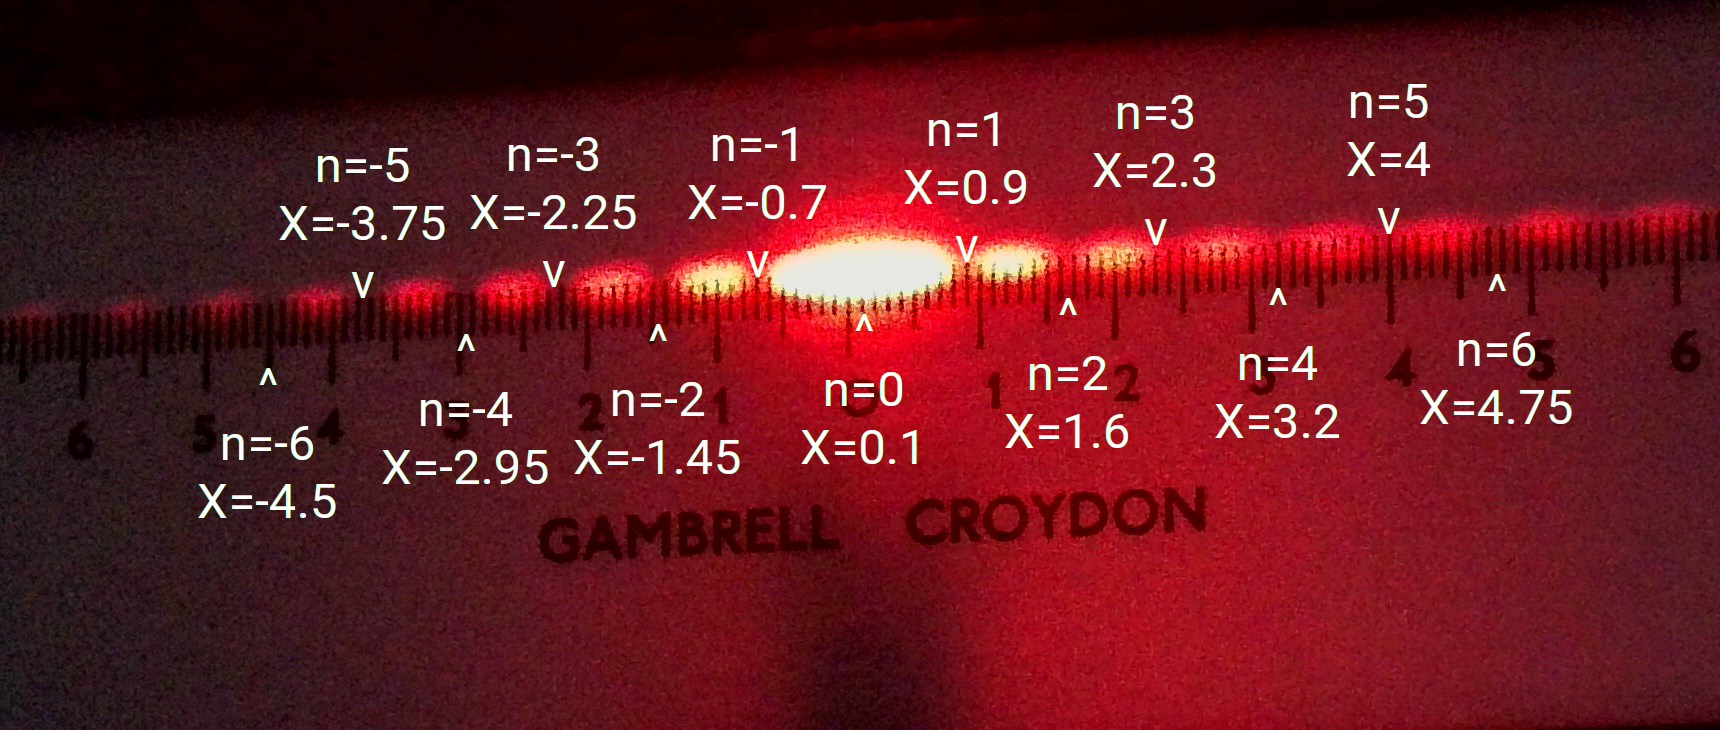
\includegraphics[scale=0.6]{L166pm1b.png}}
\caption{Analysis of the data from image {\lstinline$Q2\_slitB3.jpg$}, identifying interference minima between $N=-6$ and $N=6$, as well as $N=0$ for the $\Delta\theta$ offset}
\label{fig:l116pm1b}
\end{figure}
\newpage
For this second dataset, we obtain the following data:

\begin{table}[h!]
\centering
\begin{tabular}{ccc}
\hline
N (order) & Minima position X (cm) & Uncertainty (cm)\\ \hline
-6 & -4.5 & 0.05 \\
-5 & -3.75 & 0.05 \\
-4 & -2.95 & 0.05 \\
-3 & -2.25 & 0.05 \\
-2 & -1.45 & 0.05 \\
-1 & -0.7 & 0.05 \\
0 & 0.1 & 0.1 \\
1 & 0.9 & 0.05 \\
2 & 1.6 & 0.05 \\
3 & 2.3 & 0.05 \\
4 & 3.2 & 0.05 \\
3 & 4.0 & 0.05 \\
4 & 4.75 & 0.05 \\
\end{tabular}
\caption{\label{tab:l116b_table}Results from analysis of Figure \emph{4}}
\end{table}

With these data sets, we can fit each data point to the function described by Equation \emph{3}. By doing this, we can obtain a value for $a$, the slit width, for each of the two data sets. We employ the method of reducing the least-squares, provided by SciPy's \lstinline$curve_fit$ method. 

\begin{figure}[h!]
\centerline{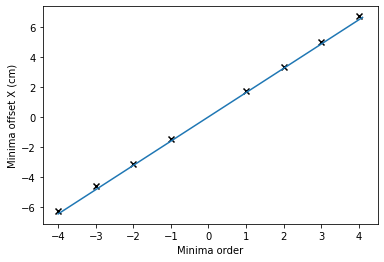
\includegraphics[scale=0.7]{L166plot.png}}
\caption{Data from Table \emph{1} fitted to the function described in Equation \emph{3}.}
\label{fig:l116plot}
\end{figure}
\newpage
\begin{figure}[h!]
\centerline{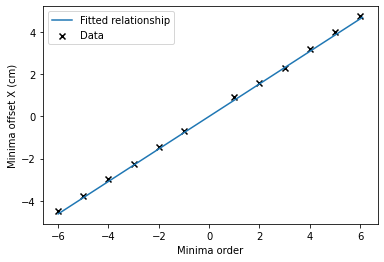
\includegraphics[scale=0.7]{L166bplot.png}}
\caption{Data from Table \emph{2} fitted to the function described in Equation \emph{3}.}
\label{fig:l116bplot}
\end{figure}

From this curve-fitting method, we obtain two values of $a$, the slit width, for image A3 ($a=64.1\mu m$) and B3 ($a=134.4\mu m$).

\section{Double Slit}
\subsection{Method}

Similarly to single slit apertures, double slit diffraction patterns can be described with a function:

\begin{equation}
\frac{I(\theta)}{I_0}=\left(\frac{\sin^2\alpha}{\alpha^2}\right)\cdot\cos^2\beta
\end{equation}

Where $\alpha=\frac\pi\lambda a\sin\theta$ (as in Equation \emph{1}) and $\beta=\frac\pi\lambda d\sin\theta$, $d$ being the distance between the middle of the two slits. The $\sin$ term can be recognised as single-slit diffraction contributions, from Equation \emph{1}, but we also account for a $\cos$ term describing the interference between the two slits. The $\sin$ term produces an "envelope" of the diffraction pattern, inside which there are smaller peaks from the $\cos$ contribution. This is demonstrated in Figure \emph{7}.

\begin{figure}[h!]
\centerline{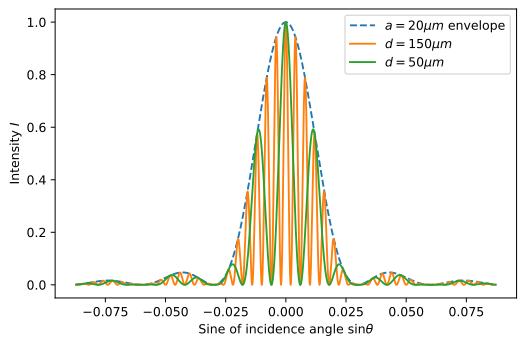
\includegraphics[scale=0.6]{double.png}}
\caption{Diagram showing the double-slit Fraunhofer diffraction patterns for 50, and 150 $\mu m$, and the envelope produced by the single-slit contribution.}
\label{fig:doubledemo}
\end{figure}

This demonstrates the observation of "missing" maxima, where the double-slit peak is cancelled out by the single-slit envelope. 
\newpage
\subsection{Data and Analysis}

By analysing the data provided in image \lstinline$Q4_double_slit_4.jpg$, we can identify the interference minima. We will only do this for the for the first envelope.

\begin{figure}[h!]
\centerline{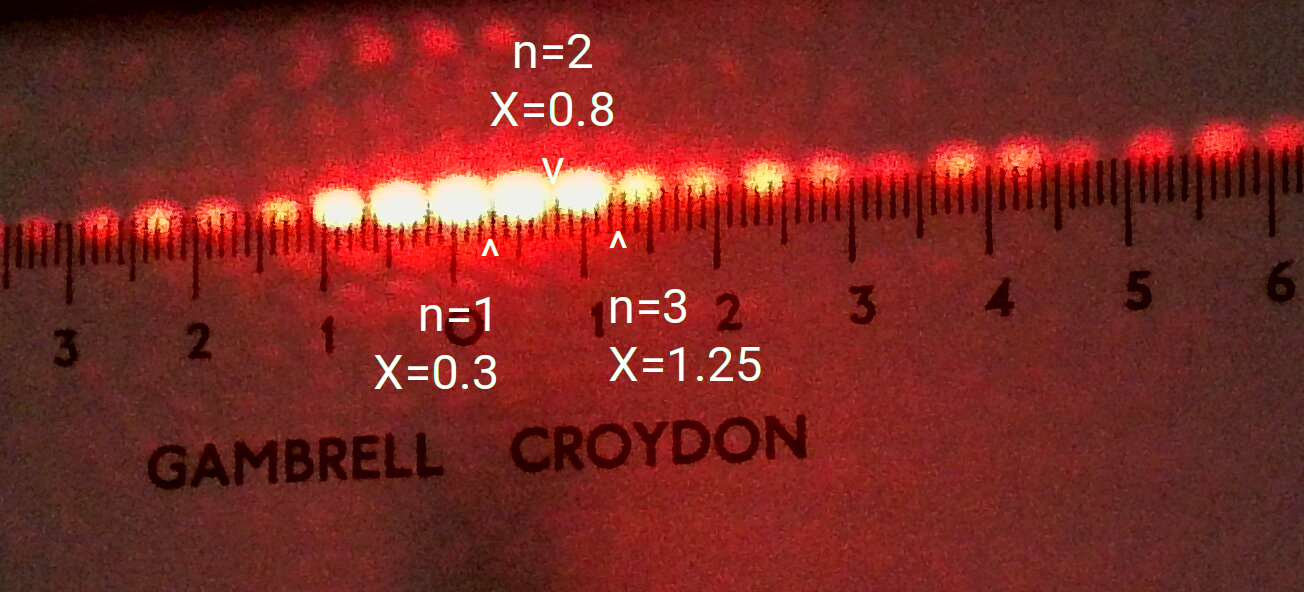
\includegraphics[scale=0.95]{doubleslit.png}}
\caption{Analysis of the data from image {\lstinline$Q4_double_slit_4.jpg$}, identifying three diffraction minima.}
\label{fig:doubleslit}
\end{figure}

From analysing where zeroes occur both products of Equation \emph{4}, we can see that the $\cos^2\beta$ term is the contribution for these small minima, and the $\text{sinc}^2 \alpha$ term contributes to the missing maxima.

Extracting the data from the photo analysis, we obtain these results:

\begin{table}[h!]
\centering
\begin{tabular}{ccc}
\hline
N (order) & Minima position X (cm) & Uncertainty (cm)\\ \hline
1 & 0.3 & 0.01 \\
2 & 0.8 & 0.01 \\
3 & 1.25 & 0.01 \\
\end{tabular}
\caption{\label{tab:l116b_table}Results from analysis of Figure \emph{8}}
\end{table}
\newpage
From the $\cos^2\beta$ term above, we know that minima are described by the following equation, similar to that of single-slit:

\begin{equation}
\frac XL = \left(\frac{\lambda n}{d}\right)
\end{equation}
Using this, we calculate values of $L$, the distance from the slits to the screen, for orders $N=1, 2, 3$ as $1.202m$, $1.603m$, and $1.670m$ respectively. This gives us an average of $1.49m$. However, the standard deviation for this average is very high, so ideally we would repeat this measurement for all of the minima.

\section{Diffraction Grating}
\subsection{Method}

For diffraction gratings of $N$ number of slits, we use a new equation for the intensity at a given angle:
\begin{equation}
\frac{I(\theta)}{I_0}=\left(\frac{\sin^2\alpha}{\alpha^2}\right)\frac{\sin^2(N\beta)}{N^2\sin^2\beta}
\end{equation}
Where, again, $\alpha=\frac\pi\lambda a\sin\theta$ and $\beta=\frac\pi\lambda d\sin\theta$. We can demonstrate the effect of increasing the value of $N$ with plots showing $N=1, 2, 3, 10$:
\begin{figure}[h!]
\centerline{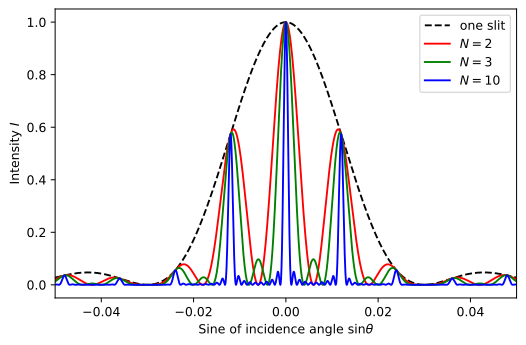
\includegraphics[scale=0.7]{grating.png}}
\caption{Diagram showing the diffraction grating Fraunhofer diffraction patterns for $a=20\mu m$, $d=50 \mu m$, and values of $N$ $1, 2, 3, 10$.}
\label{fig:gratingdemo}
\end{figure}
\newpage
\subsection{Data and Analysis}
We can also see how the grating spacing $d$ effects the patterns, using the two examples provided; {\lstinline$Q6_gratingA.jpg$} and {\lstinline$Q6_gratingB.jpg$}:

\begin{figure}[h!]
\centering
\begin{subfigure}{.5\textwidth}
	\centering
	\centerline{\includegraphics[scale=0.25]{gratinga.png}}
	\caption{{\lstinline$Q6_gratingA.jpg$}}
\end{subfigure}%
\begin{subfigure}{.5\textwidth}
	\centering
	\centerline{\includegraphics[scale=0.25]{gratingb.png}}
	\caption{{\lstinline$Q6_gratingB.jpg$}}
\end{subfigure}
\label{fig:gratings}
\caption{The two provided images of diffraction gratings.}
\end{figure}

We can see that Figure \emph{10a} has more maxima fringes than Figure \emph{10b}, spaced close together. This tells us, qualitatively, that {\lstinline$Q6_gratingA.jpg$} has a larger grid spacing $d$ than {\lstinline$Q6_gratingB.jpg$}

When these grids are superimposed perpendicularly, they form a "lattice" of rectangles. Diffraction causes these rectangles to "invert" when projected to a screen, as shown in this diagram:

\begin{figure}[h!]
\centering
\centerline{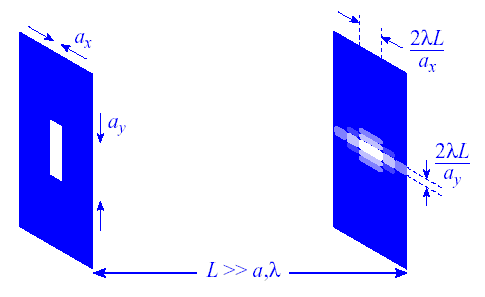
\includegraphics[scale=0.5]{rectangles.png}}
\caption{Diagram showing how rectangular apertures diffract. \\Image sourced from {\lstinline$electron9.phys.utk.edu/optics421$}} 
\label{fig:rectangles}
\end{figure}

This means that we can qualitatively determine the orientation of these gratings from their pattern. In the image below, we see that the shorter $"x"$ dimension is orientated around 25 degrees from the zenith. This means that the slits of Grating $B$, with closer grid spacings than Grating $A$, are orientated 25 degrees clockwise from the zenith. 
\newpage
\begin{figure}[h!]
\centering
\centerline{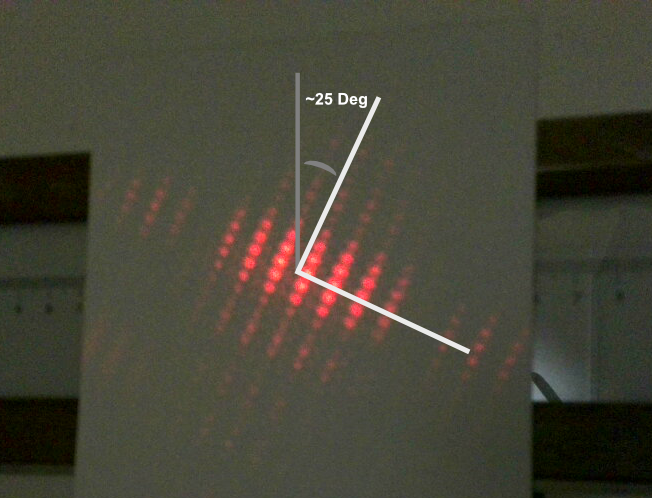
\includegraphics[scale=0.5]{perp.png}}
\caption{{\lstinline$Q7_perp_gratings_1.jpg$} modified to include the orientations of the diffraction gratings.} 
\label{fig:perp}
\end{figure}

Image {\lstinline$Q7_perp_gratings_2.jpg$} has been rotated a further 90 degrees, {\lstinline$Q7_perp_gratings_3.jpg$}, and has been rotated 25 degrees \emph{anti}-clockwise from the zenith. {\lstinline$Q7_perp_gratings_4.jpg$} has been rotated around 45 degrees from the zenith, and {\lstinline$Q7_perp_gratings_5.jpg$} has not been rotated, with the slits from grating $B$ pointing directly upwards.

\section{Circular Apeture}
\subsection{Method}
For Fraunhofer diffraction in a uniform circular apeture, we get a new equation to describe the intensity:
\begin{equation}
\frac{I(\theta)}{I_0}=\left(\frac{2J_1(z)}z\right)^2
\end{equation}
Where $z=\frac\pi\lambda d\sin\theta$, and $J_1$ is the first-order Bessel function. This is known as an Airy pattern, and produces concentric rings. We are also provided a list of the first 6 orders of where $J_1(z_i)=0$: $z_1 = 3.832$, $z_2 = 7.016$, $z_3 = 10.173$, $z_4 =
13.324$, $z_5 = 16.471$, $z_6 = 19.616$. 

From Equation \emph 7 we can then also determine the diameters $D_i$ of the $i^\text{th}$ dark ring:

\begin{equation}
D_i=\frac{2L\lambda}{\pi d}z_i
\end{equation}
\newpage
\subsection{Data and Analysis}

Using Equation \emph 8, we can measure the distance from the center of the diffraction pattern to the center of each dark ring, and use that to determine $L$, given the values for $\lambda=6.238\times10^{-7}\ m$ and $d=0.0003\ m$. 

To do this, we use the {\lstinline$Q8_pinhole6.jpg$} provided, shown below with the measurements of $D_i$ annotated:

\begin{figure}[h!]
\centering
\centerline{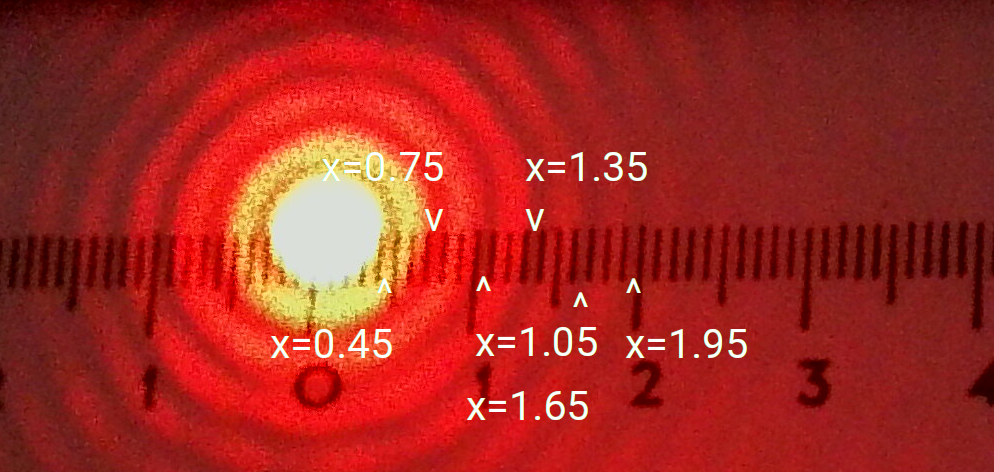
\includegraphics[scale=1.1]{pinhole.png}}
\caption{{\lstinline$Q8_pinhole6.jpg$} modified to include the measurements of $D_i$.} 
\label{fig:pinhole}
\end{figure}

The results of these measurements are tabulated below.

\begin{table}[h!]
\centering
\begin{tabular}{ccc}
\hline
n (order) & $D_i$ (cm) & $z_i$\\ \hline
1 & 0.45 & 3.832 \\
2 & 0.75 & 7.016 \\
3 & 1.05 & 10.173 \\
4 & 1.35 & 13.324 \\
5 & 1.65 & 16.471 \\
6 & 1.95 & 19.616 \\
\end{tabular}
\caption{\label{tab:pinhole_table}Results from analysis of Figure \emph{13}}
\end{table}

We now use the same method of analysis as Section \emph{2.2}; curve-fitting the experimental results with Equation \emph 8 to obtain an estimate for $L$. Using this method, we are able to obtain an estimate value of $L=0.763\ m$ for the slit-screen distance. The curve-fitting results are shown in Figure \emph{14}.

\begin{figure}[h!]
\centerline{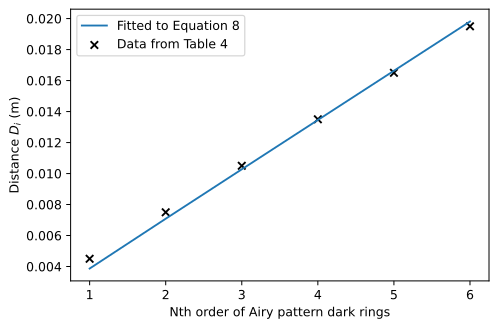
\includegraphics[scale=0.7]{pinhole_plot.png}}
\caption{Data from Table \emph 4 fitted to the function described in Equation \emph 8}
\label{fig:pinhole_plot}
\end{figure}
\newpage
\section{Fresnel Diffraction Regime}
\subsection{Method}

Up until now, we have been analysing diffraction patterns in the Fraunhofer regime. However, when the viewing screen is considerably closer to the source than in the Fraunhofer regime, we enter the Fresnel regime where the wavefronts have significant curvature over the geometry of the aperture. We have a quantitative condition for the Fraunhofer regime:
\begin{equation}
\frac{a^2}{L\lambda}\ll 1
\end{equation} 
Where $a$ is the aperture size and $L$ is the slit-screen distance. In our single-slit experiments in Section \emph{2.1}, and Young's double-slit experiments in Section \emph{3.1}, we can prove that this condition is satisfied, and so in the Fraunhofer (far viewing screen) regime.
\subsubsection{Single Slit}
In our single-slit experiments, we had a slit-screen distance of $L=1.66\pm 0.01\ m$, and aperture sizes of $a_1=6.41\times 10^{-5}\ m$ and $a_2=1.344\times1-^{-4}\ m$. In both of these conditions, our values from Equation \emph 9 are:
\begin{equation}
\frac{a_1^2}{L\lambda}=\frac{(1.41\times10^{-5})^2}{1.66\cdot6.238\times10^{-7}}=0.00019...\ll 1
\end{equation}%
and:
\begin{equation}
\frac{a_2^2}{L\lambda}=\frac{(1.344\times10^{-4})^2}{1.66\cdot6.238\times10^{-7}}=0.01744...\ll 1
\end{equation}
From this, we can see that the Fraunhofer regime conditions are satisfied for both scenarios.
\subsubsection{Double Slit}
In the double-slit experiments, we had a set-up with single-slit widths $a\approx6\times10{-5}\ m$, and calculated an average slit-screen distance $L=1.49\ m$. In this condition, our values from Equation \emph 9 are:
\begin{equation}
\frac{a^2}{L\lambda}=\frac{(6\times10^{-5})^2}{1.49\cdot6.238\times10^{-7}}=0.00387...\ll 1
\end{equation}
From this, we can see that the Fraunhofer regime condition is satisfied.
\subsection{Qualitative Analysis}
In Section \emph{5.2}, we studied spherical aperture diffraction in the Fraunhofer regime. Historically, when Fresnel proposed his new "wave-theory" of light in 1818, it was largely ridiculed by scientists at the time, preferring Newton's "corpuscular" theory of light. Poisson noted that, as a consequence of Fresnel's theory, one could predict that under some conditions, the theory predicted a bright spot at the central point of a spherical shadow, and a dark spot at the central point of a circular aperture. Since this was not commonly observed, Poisson saw this as a flaw and dismissed the theory. Arago however modelled these such conditions, with a $2\ mm$ metallic disk, and prove this dark/light spot. This came to be known as Poisson's spot, despite observations a century earlier by Delisle and Maraldi. 

We too can observe this phenomena. When the laser beam source is first passed through a lens, it causes the wavefronts to enter the spherical condition for Fresnel regime diffraction. We can analyse photographs of our existing experimental set-ups, one including this lens and one, to observe the Poisson's spot appearing in Figure \emph{15b} when moving between regimes.

\begin{figure}[h!]
\centering
\begin{subfigure}{.5\textwidth}
	\centering
	\centerline{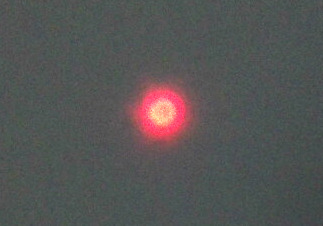
\includegraphics[scale=2.33]{poissonB.png}}
	\caption{{\lstinline$Q10_fresnelB1.jpg$}}
\end{subfigure}%
\begin{subfigure}{.5\textwidth}
	\centering
	\centerline{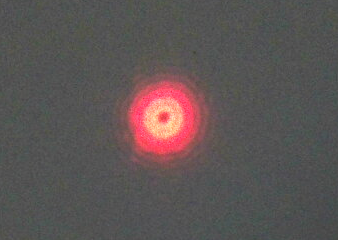
\includegraphics[scale=2.22]{poissonA.png}}
	\caption{{\lstinline$Q10_fresnelA1.jpg$}}
\end{subfigure}
\label{fig:poisson}
\caption{Two provided images of spherical aperture diffraction, cropped, showing the transition from Fraunhofer regime to Fresnel regime, and the observation of Poisson's spot in Figure \emph{15b}.}
\end{figure}

\end{document}
